%----------------------------------------------------------------------------
\chapter*{Bevezető}\addcontentsline{toc}{chapter}{Bevezető}
%----------------------------------------------------------------------------

% Gyakorlás szerepe a tanulásban
A tanulás egy nehéz és időigényes folyamat, melynek megértésével és tökéletesítésével napjainkban is aktívan foglakozik a tudomány.
Ennek a folyamatnak elengedhetetlen része az önállóan végzett feladatmegoldás, a gyakorlás, mely során az elméleti tudás a gyakorlatban is hasznosítható tapasztalattá válik.
Gyakorlás közben fontos, hogy minél gyakrabban -- ha lehet, folyamatosan -- ellenőrizzük munkánk eredményét, ezzel biztosítva azt, hogy ne keletkezzenek rossz berögződések, melyek utólagos kijavítása további időt igényelne.

Az ellenőrzésnek sokféle módja is ismert, mely módozatokat többféle nézőpontból is értékelhetünk.
Az egyik ilyen nézőpont az ellenőrzési módszer flexibilitása, amely azt mutatja meg, mennyire változtatható meg a feladat úgy, hogy az ellenőrzési módszer továbbra is alkalmazható maradjon.
A spektrum egyik végén állnak az inflexibilis módszerek, amilyen például egy adott feladathoz mellékelt megoldókulcs.
A legegyszerűbb megoldókulcsok egyedül a feladat elvárt eredményét adják meg, ezért ezek flexibilitása igen csekély, hiszen a feladatban bármilyen érdemi változtatást elvégezve elvesztik érvényességüket. 
Ugyanakkor ezek a leggyorsabb és legolcsóbb módszerek, hiszen egyetlen összehasonlítás szükséges a saját és a megoldókulcs által megadott érték között, a megoldókulcsok pedig minimális költséggel sokszorosíthatóak és felhasználhatóak.
A spektrum másik végén találhatóak a flexibilis módszerek, amilyen például az oktatók -- általános esetben az adott terület szakértőinek -- alkalmazása, akik a feladat témakörében való jártasságuk révén gyakorlatilag bármely megoldás ellenőrzésére képesek.
Az oktató azonban drága erőforrás, mind időben, mind pénzben, hiszen egy adott téma szakértőjeként a tanulók feladatainak ellenőrzése helyett az iparban is nagy szükség lenne rá.
Ebből fakadóan -- sok oktató alkalmazása költséges, ugyanakkor az iparnak nagyszámú szakértőre van szüksége -- az egy oktatóra eső hallgatók száma igen magas, amely körülmény nem kedvez az oktatás színvonalának, hiszen így minden hallgatóra kevesebb ideje jut az oktatónak.
E két véglet között megannyi módszert találunk, amelyek alkalmazhatósága nagyban függ a feladat jellegétől és témakörétől.

Az oktatók alkalmazásának van azonban egy másik nagy előnye is: a tanulók eredményessége egy független személy által is értékelésre kerül.
Enélkül az oktatási és egyéb akkreditációs intézmények legitimitása megszűnne, működésük értelmét vesztené.

Napjainkban a költségek csökkentésének és a hatékonyság növelésének egyik leggyakoribb formája még mindig az automatizálás.
Az első ipari forradalommal a világ rohamos fejlődésnek indult, melyet a második és a harmadik forradalom után most a negyedik követ \cite{FourthRevolution}.
\begin{figure}[h]
    \centering
    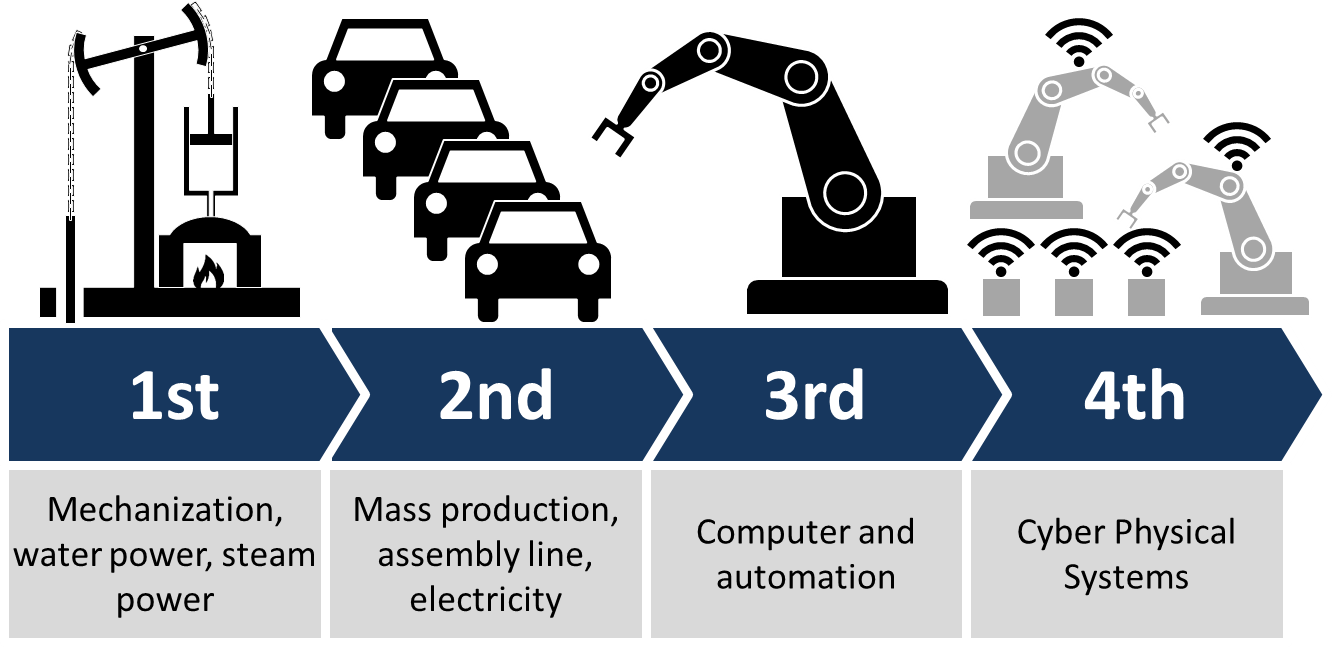
\includegraphics[width=0.8\textwidth]{figures/industrial_revolutions}
    \caption[Ipari forradalmak]{Ipari forradalmak (forrás: Christoph Roser at AllAboutLean.com)} % https://en.wikipedia.org/wiki/Industry_4.0#/media/File:Industry_4.0.png
\end{figure} 
A nagyfokú automatizálás a harmadik ipari forradalom részeként a számítógépek elterjedésével jelent meg.
A számítógépek lehetővé teszik olyan feladatok automatizálását is, melyek azelőtt lehetetlennek tűntek, ráadásul mindezt egyre olcsóbban.

Ha a számítógépek által nyújtott automatizálás tulajdonságait -- olcsó hardver, könnyen sokszorosítható szoftver, gyors működés, akár igen magas szintű flexibilitás szakértelem (mesterséges intelligencia) hozzáadásával -- vizsgáljuk, könnyű belátni, hogy igen kedvezőek az eddig említett ellenőrzési módszerekkel összevetve.
Ezen gondolatmeneten továbbhaladva eljuthatunk az \textit{automatizált ellenőrzőrendszerek} ötletéhez.
Az automatizált ellenőrzőrendszerek olyan számítógépes szoftverek, melyek a szakértők által előre betáplált logika segítségével képesek bizonyos feladatcsoportok megoldásainak ellenőrzésére.
Ezek a rendszerek különösen jól alkalmazhatóak azokon a területeken, ahol a feladatok helyes megoldásai egyszerű szabályrendszerekkel leírhatóak, ellenőrizhetőek.
Az egyik ilyen terültet a programozás oktatása, ami a dolgozat alapját adó feladatkiírásban is szerepel.

A harmadik ipari forradalom óta, de különösen a negyedik hajnalán, az iparban egyre nagyobb igény mutatkozik informatikai szakemberek iránt, mely az utóbbi években hiányszakmává nőtte ki magát az utánpótlásképzés lassúsága miatt.
A szükséges informatikusok nagy részét programozóként alkalmaznák, és szinte mindegyiküknek legalább érintőlegesen ismerniük kell a programozás alapjait.
A szakemberek képezésének hatékonyságát növelhetjük, ha az oktatókra nehezedő teher egy részét levesszük a vállukról automatizálás segítségével, illetve a tanulni vágyókat is segítjünk, hogy könnyebben hozzájuthassanak a tanuláshoz szükséges erőforrásokhoz.

\section*{Tanulás menedzsment rendszerek}\addcontentsline{toc}{section}{Tanulás menedzsment rendszerek}
A tanulás menedzsment rendszerek (learning management systems, LMS) olyan elektronikus oktatást (e-learning) támogató szoftveralkalmazások, melyek funkciói az oktatás minden aspektuásra kiterjed(het)nek.
Ezek a funkciók általában az alábbiakra terjednek ki:
\begin{itemize}
    \item tananyag szolgáltatás
    \item hallgató-regisztárció és -adminisztráció
    \item oktatási események menedzsmentje (pl. tanórák, számonkérések)
    \item tanterv és minősítés menedzsment
    \item készség és kompetencia menedzsment
    \item egyéni tanterv készítése
    \item értékelés és nyilvántartás
    \item jelentéskészítés
    \item képzési adatok menedzselése
    \item erőforrás menedzsment
    \item kurzuskészítés
\end{itemize}
Bár ilyen jellegű szoftvereket már az 1970-es években is fejlesztettek, széleskörű elterjedésük azonban csak az utóbbi évtizedben kezdődött meg az olcsó személyi számítógépek és szélessávú internet hozzáférések megjelenésével párhuzamosan.
A 2000-es évek eleje óta rengeteg elektronikus távoktatással foglalkozó vállalkozás jelent meg az interneten (pl. Coursera, Khan Academy, edX), melyeken a legnagyobb oktatási intézményeket is megszégyenítő mennyiségben gyűltek össze változatos tananyagok, melyeket akár egy kattintással elérhet a felhasználó.
A ma is használt rendszerek többsége webes felületet használ arra, hogy eljuttassa a tartalmakat a felhasználókhoz, mivel ez egyszerűen, legtöbbször telepítés nélkül elérhető minden elterjedt operációsrendszeren.
A tananyagok tartalmazhatnak hagyományos, tankönyvekhez hasonló, statikus, többségében szöveges, néhol képekkel kiegészített tartalmakat, vagy akár modernebb, audióvizuális, esetleg interaktív anyagokat is.
% NOTES: video konferencia, szabad bővíthetőség
Léteznek ingyenes, fizetős, illetve a kettő között sokféle konstrukcióban elérhető szolgáltatások és platformok is.

Ahogy az informatika más szegmenseiben, úgy itt is igaz, hogy a zárt forrású, fizetős szolgáltatások és rendszerek minősége jobb, mint ingyenes és/vagy nyílt forrású társaiké.
Szerencsére ez az állapot az utóbbi pár évben javulú tendenciát mutat, hiszen egyre több, eddig zárt forrású szoftvereket készítő cég teszi nyílt forrásúvá szoftvereit, felismerve a közösségi fejlesztésben rejlő előnyöket és lehetőségeket (pl. Open edX), de jelenleg a piacon még többségben vannak a zárt forrású megoldások.

Az eddig említett tanulás menedzsment rendszerek többségére igaz, hogy fejlesztőik egy általánosan használható platform kialakítására törekedtek, amely nem részesíti előnyben egyik tudományterületet sem.
Ennek a megközelítésnek a hátránya, hogy nem rendelkeznek szakterület specifikus modulokkal, melyek egy adott tudományterület oktatását olyan módszerekkel támogathatnák, amik más területeken nem alkalmazhatóak.
Ilyen modul lehetne a feladatkiírásban említett \textit{feladatkiértékelő alrendszer}.

\section*{Feladatkiértékelő rendszer}\addcontentsline{toc}{section}{Feladatkiértékelő rendszer}
\textbf{Feladatkiértékelő rendszer} alatt jelen dolgozatban olyan automatizált ellenőrzőrendszert értünk, amely a hallgatók gyakorlati feladatokra adott megoldásait számítógéppel, automatizáltan ellenőrzi, értékeli, és az értékelését megjeleníti a hallgató és az oktatók számára.
Az elnevezés elsőre kissé félrevezető lehet, hiszen nem egy adott feladatot megoldó -- kiértékelő --, hanem a feladatra adott hallgatói megoldás helyességét ellenőrző rendszerről van szó, amely az ellenőrzés végén a megoldást \textit{értékeli} is.

Diplomamunkám során egy ilyen kiértékelő modul megtervezése volt a feladatom az Irányítástechnika és Informatika Tanszék számára készített JPORTA elnevezésű, oktatást támogató portálhoz.

\section*{A diplomaterv felépítése}\addcontentsline{toc}{section}{A diplomaterv felépítése}
A dolgozat \ref{chapter:jporta}. fejezetében ismertetem a JPORTA rendszer történelmi előzményeit, bemutatom lényegesebb funkcióit, használatát oktatói és hallgatói szempontból.

A \ref{chapter:exercise}. fejezet a feladatleíró és -kiértékelő modullal foglalkozik.
Először a tervezés megkezdéséhez elengedhetetlen, a modul funkcionalitásával kapcsolatos igényfelmérést és annak eredményét részletezem, a követelmények megfogalmazása után pedig vázolom a megtervezendő rendszer magasszintű működését.
Ezt a koncepciót követve, először megtervezek egy, a feladatok leírására alkalmas struktúrát és bemutatom a hozzá kapcsolódó feladatkészítési munkafolyamatot.
Ezután leírom a feladatkiadás és -beadás menetét, ismertetem az ehhez szükséges elemeket.
Végül a beadások ellenőrzését és értékelését végző infrastruktúrát és annak működését mutatom be.

A \ref{chapter:features}. fejezetben javaslatot teszek két új funkció megvalósítására, melyek véleményem szerint hasznosak lehetnek a hallgatók és az oktatók számára.
Az egyik funkció egy csapatok létrehozását és adminisztrációját lehetővé tevő alrendszer, melynek szükségességére az igényfelmérés során derült fény.
A másik funkció a feladatbeadásnak a Git elosztott verziókövető rendszerrel való integrációja, mely lehetővé teszi, hogy a hallgatók közvetlenül a verziókövető rendszer ``megosztás'' funkciójával adják be megoldásaikat.

A dolgozatot az elvégzett munka és továbbfejlesztési lehetőségek összefoglalásával zárom.
